\section{Conclusion}
\begin{itemize}
    \item Start with the research question
    \item Continue with repeating the path of the research
    \item Short summary of the results and which model performed the best
    \item End with why we may not get the results we sought
    \item "It is important to further improve the model to get better results"
\end{itemize}

In this thesis we have predicted the salmon price using different analytical models. In doing so we have tested how well these different models perform, when trying to predict the price of salmon using similar commodities and macroeconomic factors. The approach we had to solving this task was to first perform a simple exploratory analysis to see if there was any needed changes to be done in the preprocessing stage. This was not the case. This was followed by four different models; ARIMA, SARIMA, SARIMAX and LSTM. 

The general findings is that the SARIMA and SARIMAX models produces quite similar predictions, and both outperform the ARIMA model. This clearly indicates that seasonality must be taken into account. When examining the SARIMAX predictions we see that the confidence interval is rather large. However, the salmon price spiked massively in the spring of 2022, so this is necessary. Therefore, simply examining whether or not the model predicts the correct movement of the price is of relevance. Although the model is not great, it is somewhat capable of catching the trends in the short term. The LSTM model seems not to be able to catch the seasonality before it reaches 52 lookback variables. This makes sens as we saw from the exploratory analysis that the seasonality is a yearly pattern. But when looking back at more then 52 weeks, we saw...

Examining the Ljung-Box test on the SARIMAX model shows that the residuals are not white noise, and that there might be some trends left to capture. ... Future research

\subsection{Plausible error source for LSTM in the low lookback ranges}:
Given that the NASDAQ gathers it data though sampeling form a large range of sales venues each week and by doing this aggregating a good average in the sampeling stack. This might cause the low lookback LSTM models to look at outliers separately and not as a part of the general trend. This might cause the model to not be able to catch the general trend in the low lookback ranges.
For further research in the topic we suggest to look to try and improve the models through either utilizing more data, and more computing power to make the ARIMA and LSTM able to catch more time consuming trends in the residuals. From the ljung-box test we see that there is almost definitely trends left to capture.

\begin{figure}[H]
    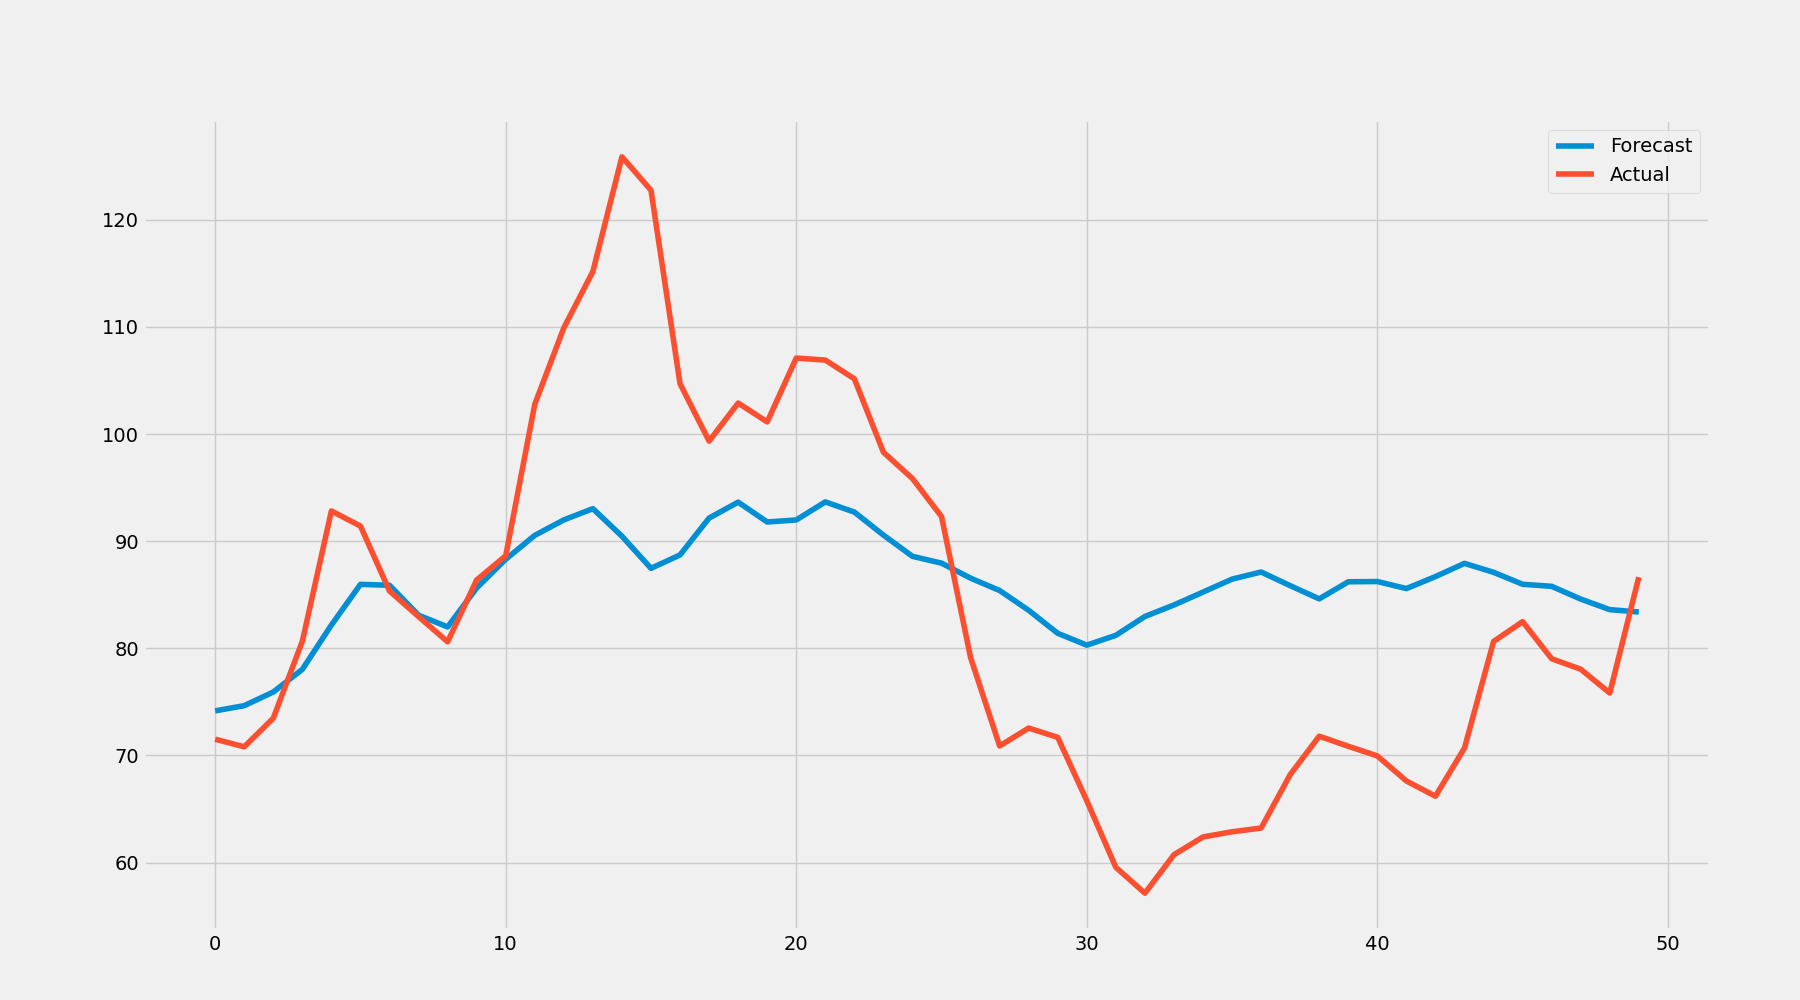
\includegraphics[width=.30\textwidth]{../data/Figures/Neural networks/ForLoop_Tensor/plotModel_186.png}\hfill
    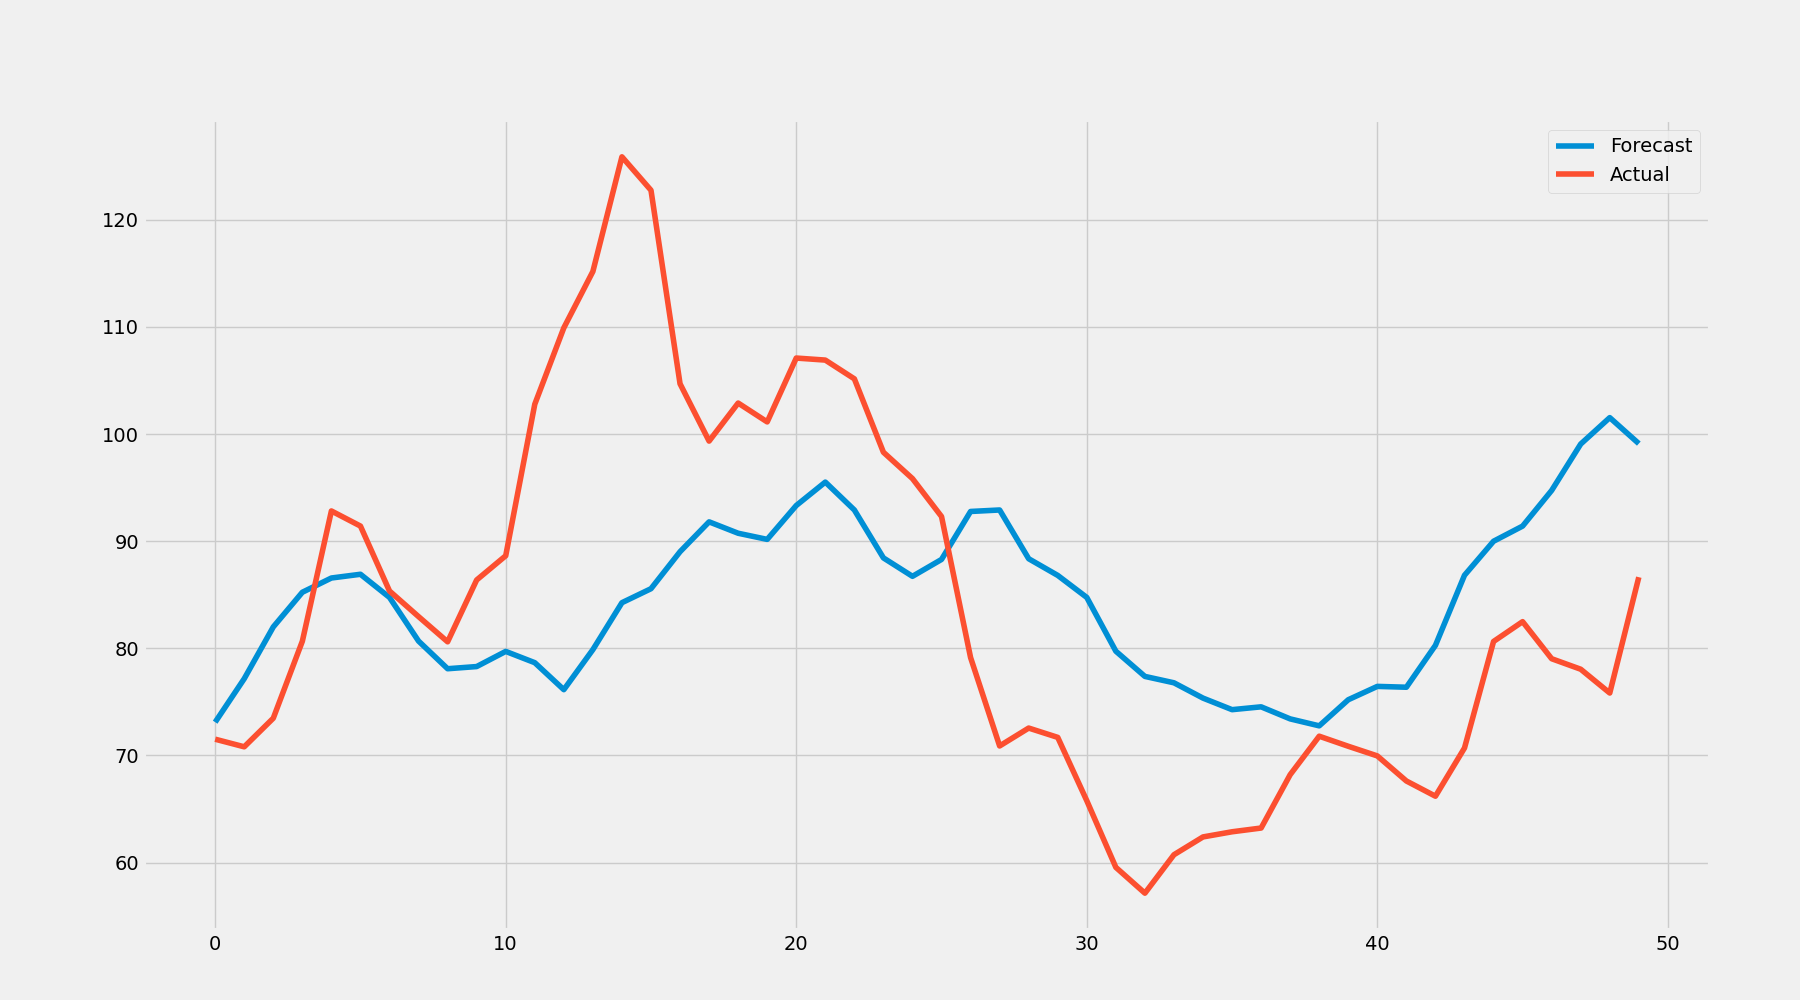
\includegraphics[width=.30\textwidth]{../data/Figures/Neural networks/ForLoop_Tensor/plotModel_72.png}\hfill
    \includegraphics[width=.30\textwidth]{../data/Figures/Neural networks/ForLoop_Tensor/plotmodel_286.png}\hfill
    \\[\smallskipamount]
    \includegraphics[width=.30\textwidth]{../data/Figures/Neural networks/ForLoop_Tensor/plotmodel_46.png}\hfill
    \includegraphics[width=.30\textwidth]{../data/Figures/Neural networks/ForLoop_Tensor/plotmodel_202.png}\hfill
    \includegraphics[width=.30\textwidth]{../data/Figures/Neural networks/ForLoop_Tensor/plotmodel_124.png}\hfill
    \\[\smallskipamount]
    \includegraphics[width=.30\textwidth]{../data/Figures/Neural networks/ForLoop_Tensor/plotmodel_130.png}\hfill
    \includegraphics[width=.30\textwidth]{../data/Figures/Neural networks/ForLoop_Tensor/plotmodel_52.png}\hfill
    \includegraphics[width=.30\textwidth]{../data/Figures/Neural networks/ForLoop_Tensor/plotmodel_268.png}\hfill
    \caption{9 best tensorflow predictions measured by RMSE}\label{fig:tensorflow preds}
\end{figure}

\begin{figure}[H]
    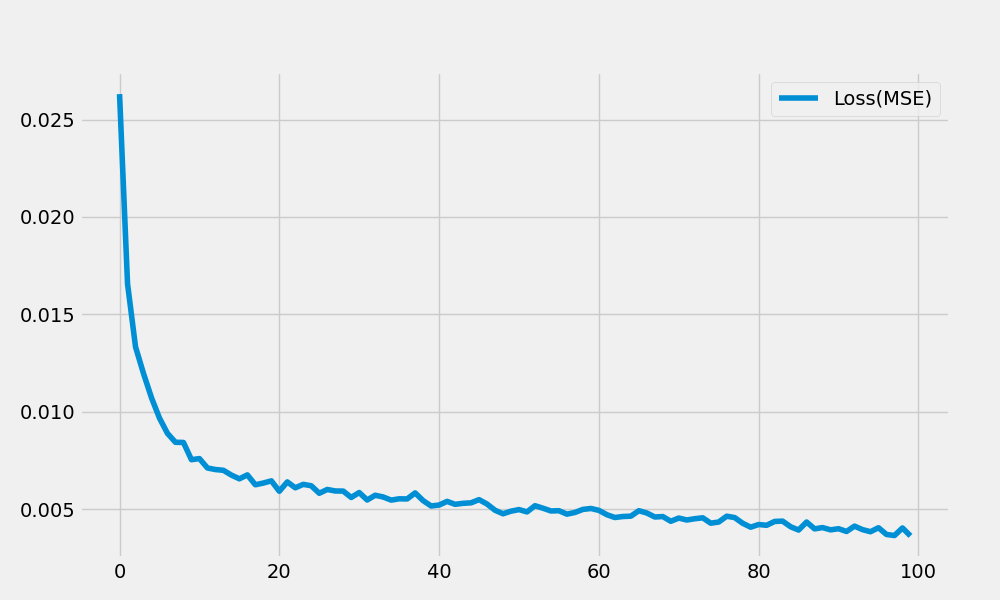
\includegraphics[width=.30\textwidth]{../data/Figures/Neural networks/ForLoop_Tensor/plotLoss_186.png}\hfill
    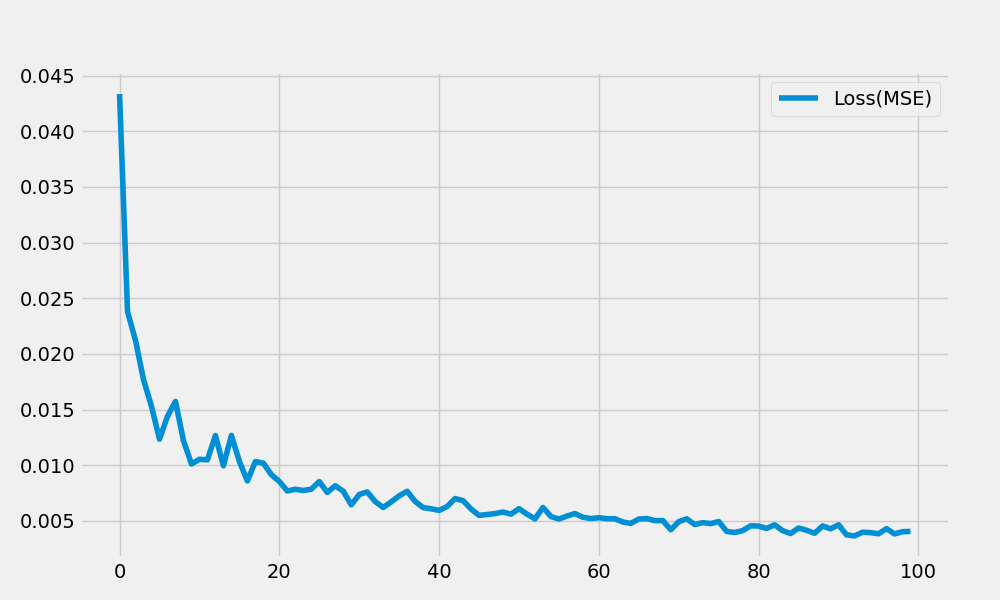
\includegraphics[width=.30\textwidth]{../data/Figures/Neural networks/ForLoop_Tensor/plotLoss_72.png}\hfill
    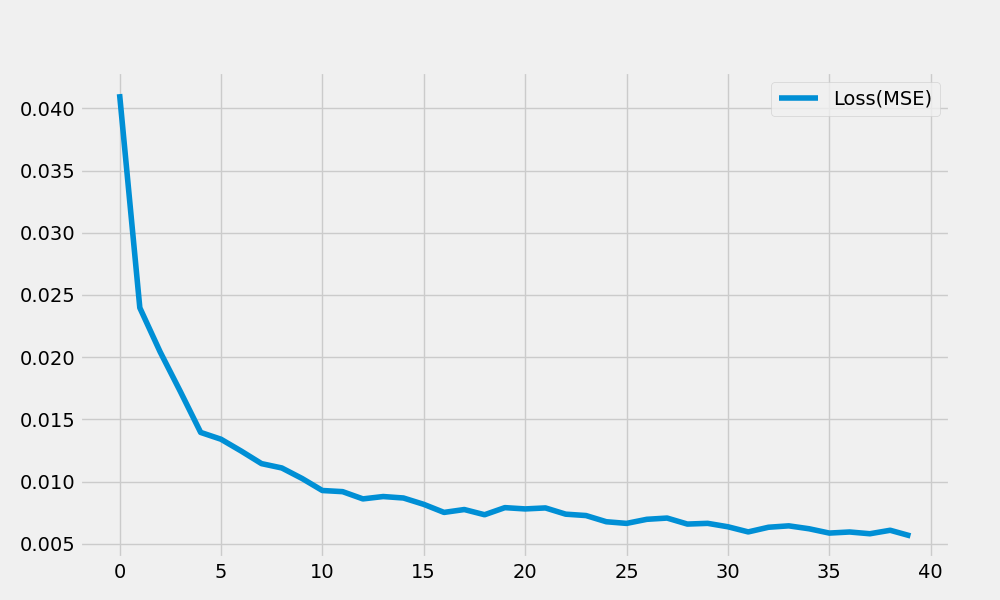
\includegraphics[width=.30\textwidth]{../data/Figures/Neural networks/ForLoop_Tensor/plotLoss_286.png}\hfill
    \\[\smallskipamount]
    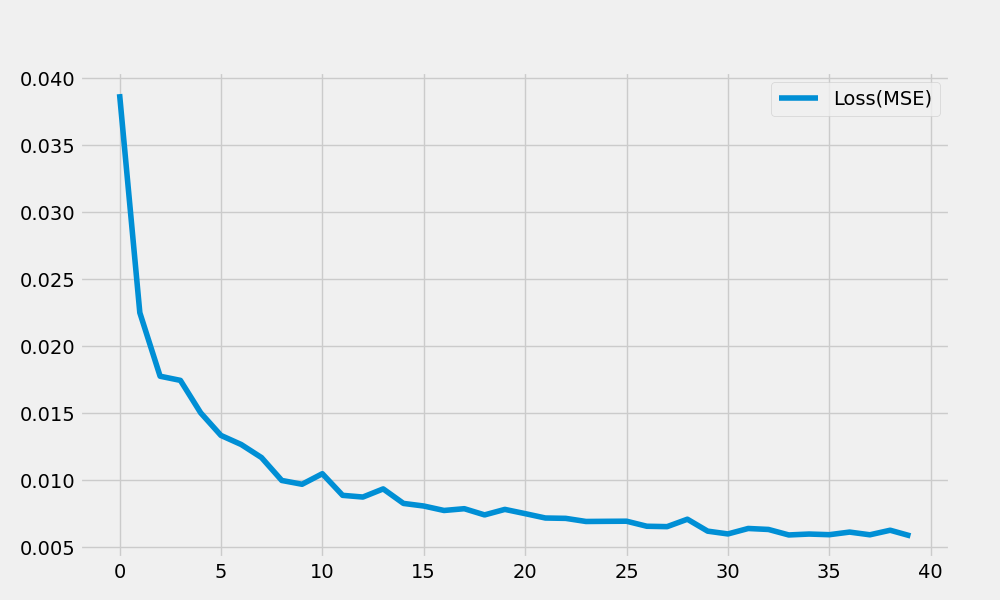
\includegraphics[width=.30\textwidth]{../data/Figures/Neural networks/ForLoop_Tensor/plotLoss_46.png}\hfill
    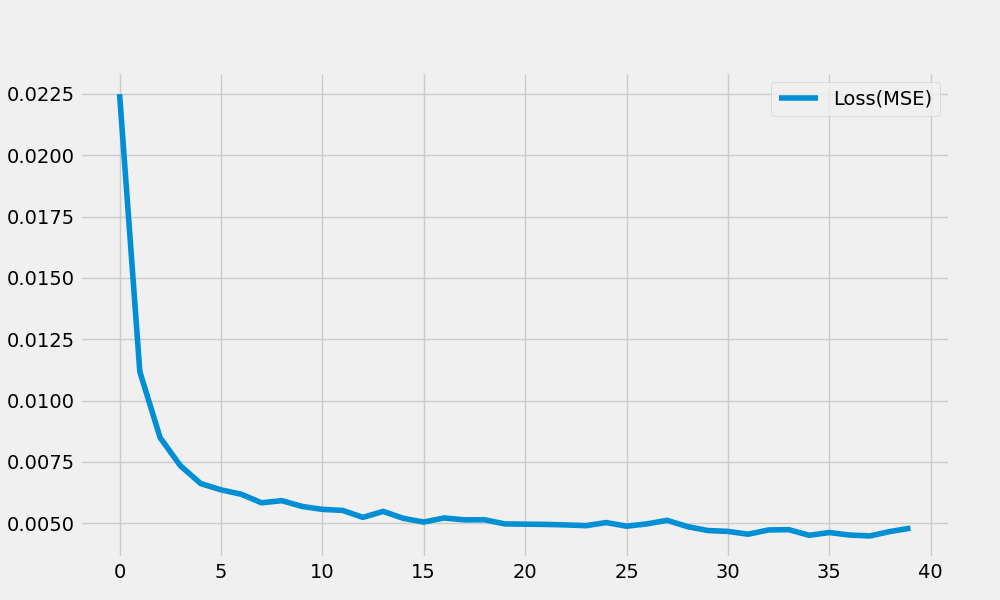
\includegraphics[width=.30\textwidth]{../data/Figures/Neural networks/ForLoop_Tensor/plotLoss_202.png}\hfill
    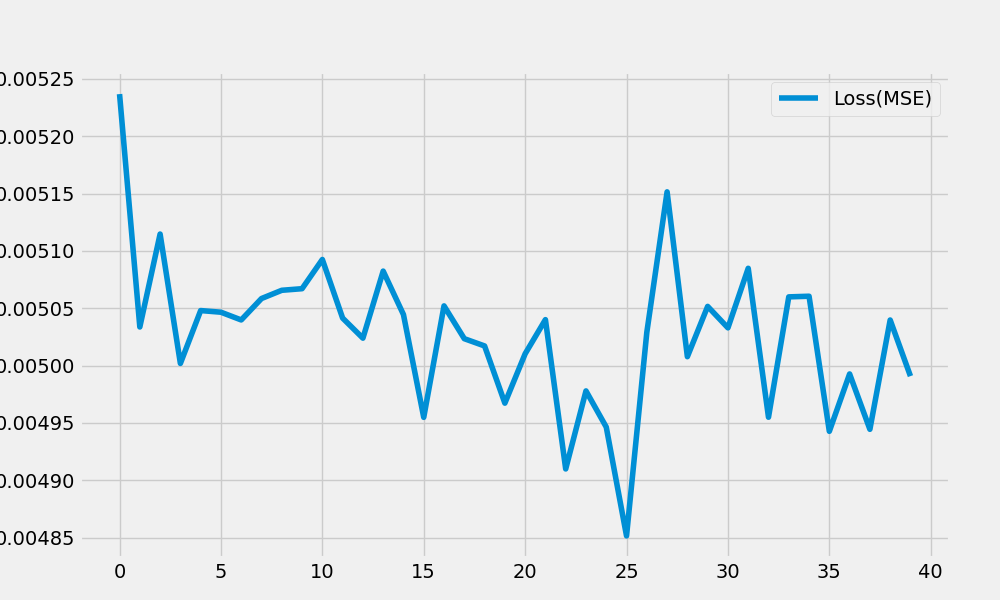
\includegraphics[width=.30\textwidth]{../data/Figures/Neural networks/ForLoop_Tensor/plotLoss_124.png}\hfill
    \\[\smallskipamount]
    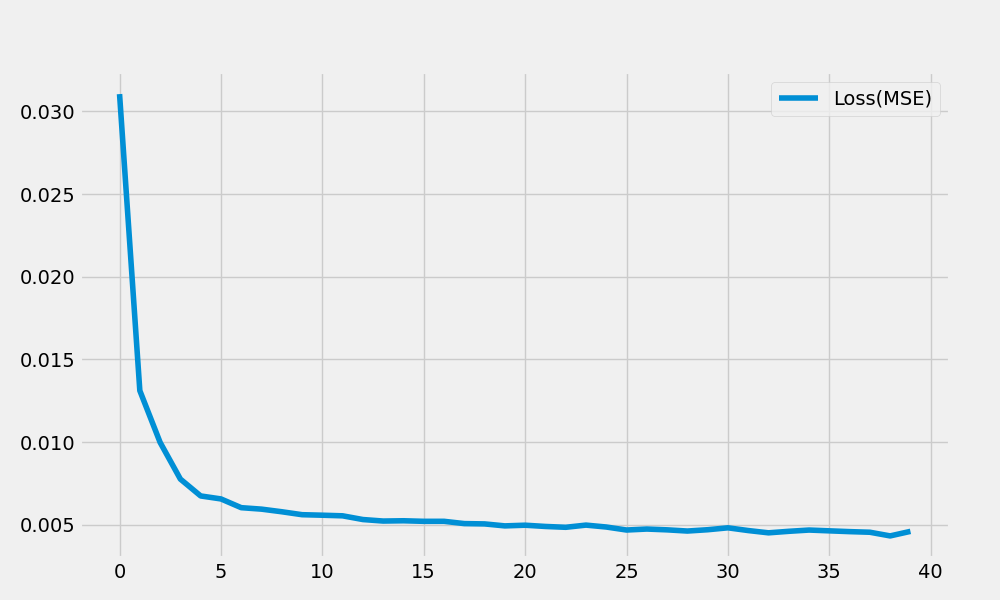
\includegraphics[width=.30\textwidth]{../data/Figures/Neural networks/ForLoop_Tensor/plotLoss_130.png}\hfill
    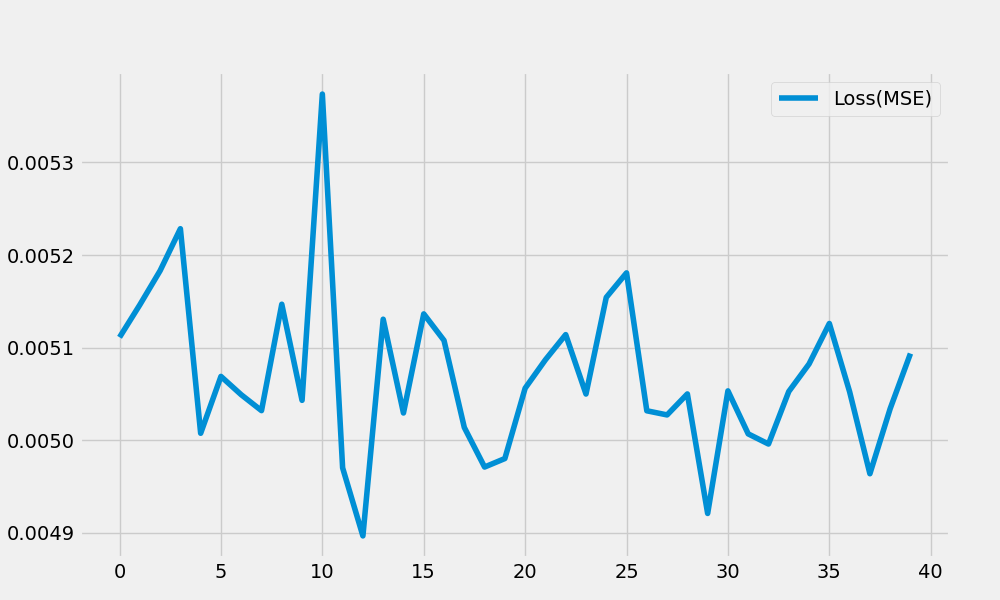
\includegraphics[width=.30\textwidth]{../data/Figures/Neural networks/ForLoop_Tensor/plotLoss_52.png}\hfill
    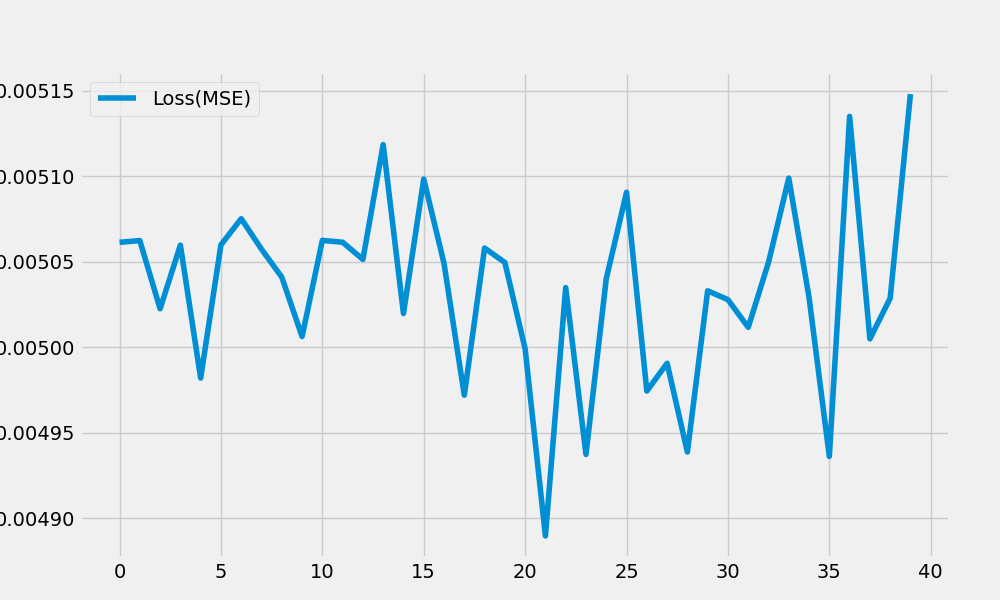
\includegraphics[width=.30\textwidth]{../data/Figures/Neural networks/ForLoop_Tensor/plotLoss_268.png}\hfill
    \caption{loss function for the 9 best tensorflow models}\label{fig:tensorflow preds loss}
\end{figure}
